\documentclass[pdflatex,sn-mathphys-num]{sn-jnl}% Math and Physical Sciences Numbered Reference Style

\usepackage{graphicx}%
\usepackage{multirow}%
\usepackage{amsmath,amssymb,amsfonts}%
\usepackage{amsthm}%
\usepackage{mathrsfs}%
\usepackage[title]{appendix}%
\usepackage{xcolor}%
\usepackage{textcomp}%
\usepackage{manyfoot}%
\usepackage{booktabs}%
\usepackage{algorithm}%
\usepackage{algorithmicx}%
\usepackage{algpseudocode}%
\usepackage{listings}%

\theoremstyle{thmstyleone}%
\newtheorem{theorem}{Theorem}%
\newtheorem{proposition}[theorem]{Proposition}% 

\theoremstyle{thmstyletwo}%
\newtheorem{example}{Example}%
\newtheorem{remark}{Remark}%

\theoremstyle{thmstylethree}%
\newtheorem{definition}{Definition}%

\raggedbottom

\begin{document}

\title[CNNs for Hand Gesture Recognition]{An Empirical Study of Convolutional Neural Networks for Hand Gesture Recognition}

\author*[1]{\fnm{Your} \sur{Name}}\email{your.email@example.com}

\affil*[1]{\orgdiv{Department of Computer Science}, \orgname{University of Milan}, \orgaddress{\street{Via Celoria 18}, \city{Milan}, \postcode{20133}, \state{MI}, \country{Italy}}}


\abstract{This paper presents a systematic approach to developing a Convolutional Neural Network (CNN) for the classification of Rock-Paper-Scissors hand gestures. Adhering to a rigorous machine learning methodology, we explore the impact of architectural complexity and regularization techniques on model performance. We design three models of increasing complexity, starting with a simple baseline and progressively introducing dropout and data augmentation. Our findings demonstrate a clear trade-off between model complexity and generalization, where the initial model exhibits significant overfitting. Regularization techniques, particularly data augmentation, prove highly effective in mitigating this issue, leading to a final model that achieves 97.7\% accuracy on an unseen test set. The study highlights the practical application of core statistical learning concepts, including the bias-variance trade-off, risk estimation, and the importance of a structured experimental process for developing robust deep learning models.}

\keywords{Convolutional Neural Networks, Image Classification, Overfitting, Regularization, Data Augmentation, Statistical Learning}

\maketitle

\section{Introduction}\label{sec1}

The task of image classification is a cornerstone of modern machine learning, with Convolutional Neural Networks (CNNs) representing the state-of-the-art approach for a wide array of visual recognition problems. This project undertakes the classification of the Rock-Paper-Scissors dataset, a collection of images depicting the three distinct hand gestures. The primary objective is not merely to maximize classification accuracy, but to conduct a methodical investigation into the process of building a robust CNN, grounded in the principles of statistical learning theory.

As outlined in the course notes \cite{cesa2024smml}, the development of a successful learning algorithm involves navigating the fundamental bias-variance trade-off. A model that is too simple may underfit the data (high bias), failing to capture the underlying patterns. Conversely, a model that is too complex may overfit (high variance), memorizing the training data, including its noise, and failing to generalize to unseen examples. This project explicitly explores this trade-off by designing, training, and evaluating three distinct CNN architectures of incremental complexity. We will analyze their performance through training curves and validation metrics, using concepts of regularization, such as Dropout and data augmentation, to control model complexity and improve generalization. The final, optimized model is then evaluated on a held-out test set to provide an unbiased estimate of its true statistical risk.

\section{Methods}\label{sec11}

Our methodology was designed to be systematic and reproducible, adhering to sound machine learning practices at every stage.

\subsection{Dataset and Preprocessing}
We utilized the Rock-Paper-Scissors dataset from Kaggle \cite{kaggle_rps}, which contains 2,188 images of hand gestures, evenly distributed across the three classes: 'rock', 'paper', and 'scissors'. The images are 300x200 pixels with varied lighting and backgrounds.

The dataset was first partitioned into three distinct, non-overlapping subsets: a training set (60\%), a validation set (20\%), and a test set (20\%). This partitioning is crucial to prevent data leakage; the validation set is used for model selection and hyperparameter tuning, while the test set is reserved for a single, final evaluation of the chosen model. All images were resized to 150x150 pixels and their pixel values were normalized from the [0, 255] range to [0, 1] by scaling with a factor of $1/255$. This normalization step is standard practice for stabilizing the training process of neural networks.

\subsection{Model Architectures}
We designed three CNN architectures with incrementally increasing complexity to study the effects on model performance and generalization. All models were implemented using the TensorFlow and Keras libraries.

\subsubsection{Model 1: Baseline CNN}
Our first model was a simple, shallow CNN designed to establish a performance baseline. Its architecture consists of a single convolutional block followed by a dense layer.
\begin{itemize}
    \item \texttt{Conv2D} (16 filters, 3x3 kernel, ReLU activation)
    \item \texttt{MaxPooling2D} (2x2 pool size)
    \item \texttt{Flatten}
    \item \texttt{Dense} (64 units, ReLU activation)
    \item \texttt{Dense} (3 units, Softmax activation for output)
\end{itemize}

\subsubsection{Model 2: Intermediate CNN with Dropout}
To address the issues observed in the baseline, the second model was made deeper and introduced regularization.
\begin{itemize}
    \item \texttt{Conv2D} (32 filters, 3x3 kernel, ReLU activation)
    \item \texttt{MaxPooling2D} (2x2 pool size)
    \item \texttt{Conv2D} (64 filters, 3x3 kernel, ReLU activation)
    \item \texttt{MaxPooling2D} (2x2 pool size)
    \item \texttt{Flatten}
    \item \texttt{Dropout} (rate of 0.5)
    \item \texttt{Dense} (128 units, ReLU activation)
    \item \texttt{Dense} (3 units, Softmax activation)
\end{itemize}
The addition of a \texttt{Dropout} layer is a key regularization technique designed to prevent overfitting by randomly setting a fraction of input units to 0 at each update during training time, which helps to make the network less sensitive to the specific weights of individual neurons.

\subsubsection{Model 3: CNN with Data Augmentation}
Our third model used the same architecture as Model 2 but was trained using data augmentation. The training data generator was configured to apply random transformations to the images in real-time:
\begin{itemize}
    \item Rotation (up to 20 degrees)
    \item Width and height shifts (up to 20\% of the dimension)
    \item Shearing and zooming (up to 20\%)
    \item Horizontal flipping
\end{itemize}
This technique artificially expands the training dataset, exposing the model to a wider variety of intra-class variations and forcing it to learn more robust and generalizable features.

\subsection{Training and Evaluation}
All models were trained using the Adam optimizer and the \texttt{categorical\_crossentropy} loss function, which is standard for multi-class classification. Performance was monitored using the accuracy metric. Hyperparameter tuning was performed on the final architecture to select an optimal learning rate, using performance on the validation set as the sole criterion.

\section{Results}\label{sec2}

The three models were trained and their performance on the training and validation sets was recorded at each epoch.

\subsection{Model 1: Baseline Performance and Overfitting}
The baseline model trained very quickly, achieving a training accuracy of 99.3\% but a peak validation accuracy of only 95.2\%. The training and validation curves, shown in Figure \ref{fig:model1}, exhibit a significant divergence, which is a classic sign of **overfitting**. The model has low bias, as it can fit the training data almost perfectly, but high variance, as it fails to generalize equally well to the unseen validation data.

\begin{figure}[h]
\centering
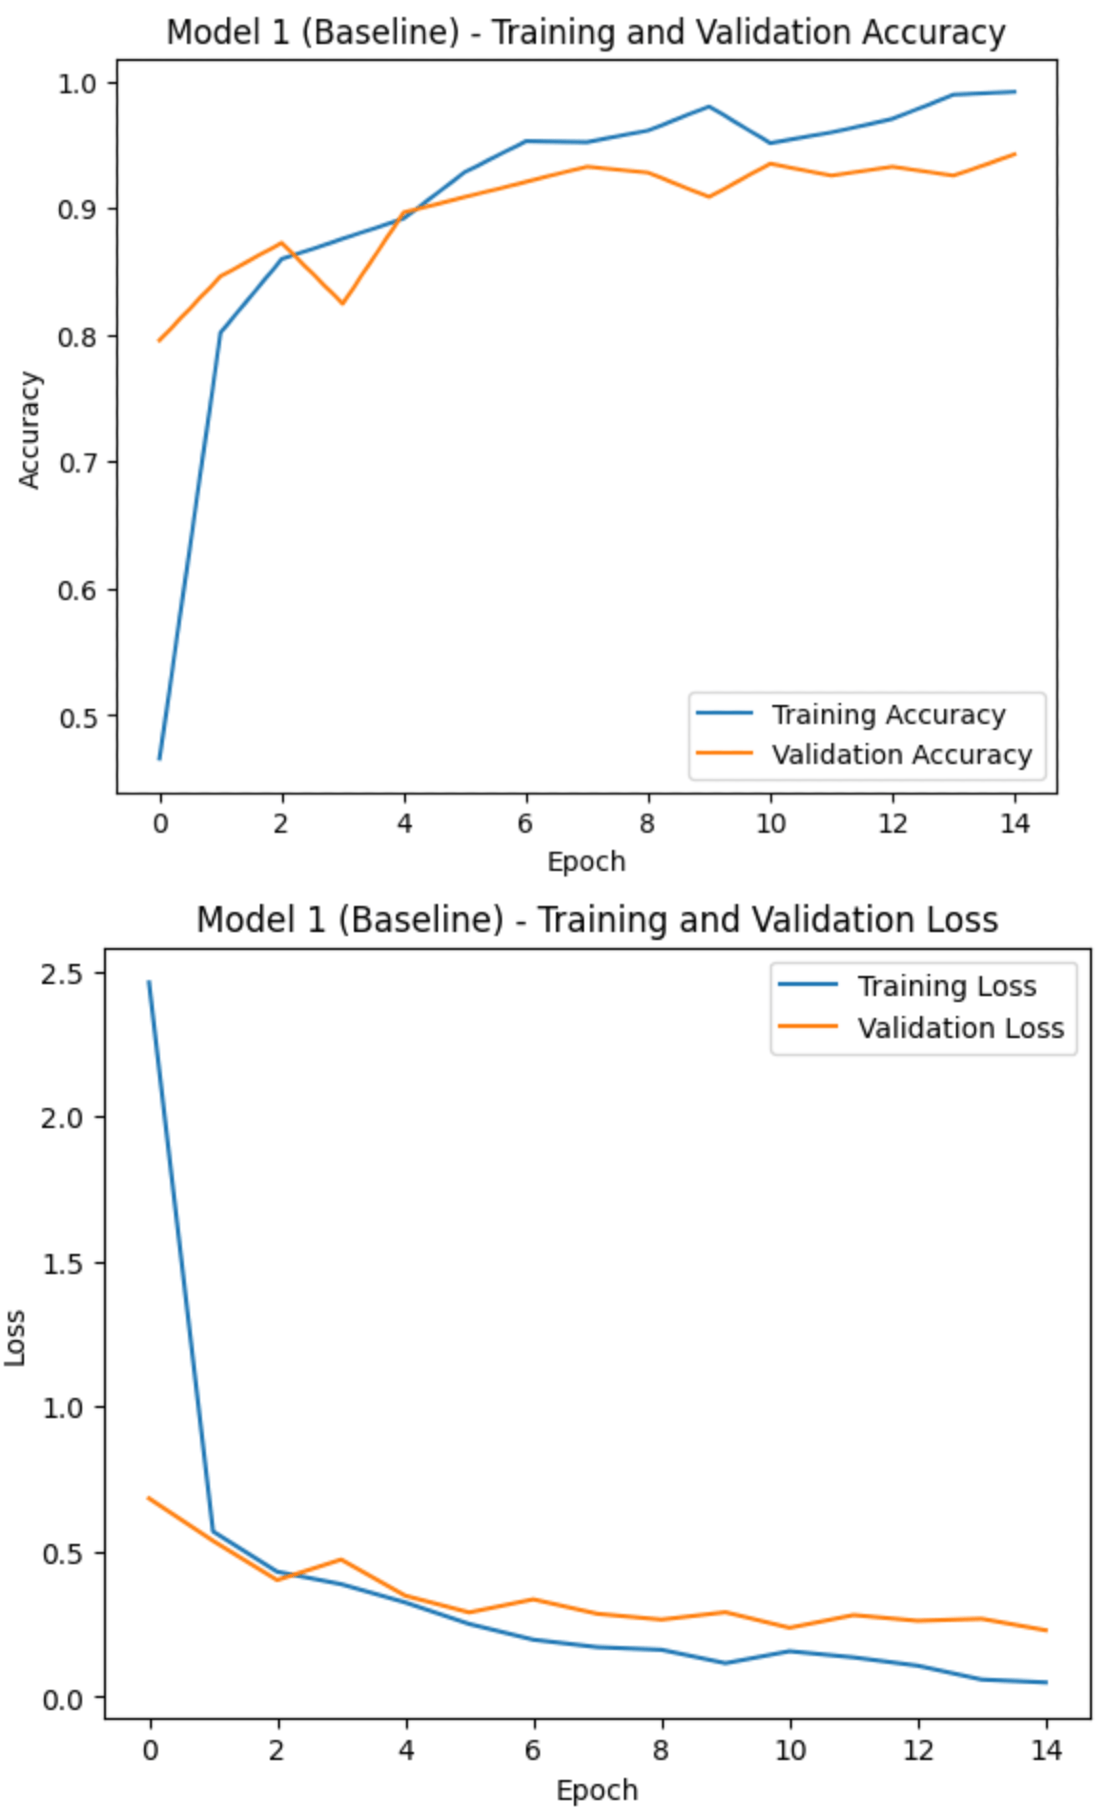
\includegraphics[width=0.9\textwidth]{model1_curves.png}
\caption{Training and validation accuracy/loss for Model 1. The growing gap between the training and validation curves indicates significant overfitting.}\label{fig:model1}
\end{figure}

\subsection{Model 2: The Effect of Dropout}
The second model, incorporating an additional convolutional block and a dropout layer, showed improved performance. It achieved a peak validation accuracy of 96.2\%. As seen in Figure \ref{fig:model2}, the gap between the training and validation curves is noticeably smaller compared to the baseline model. This demonstrates that the dropout layer successfully acted as a regularizer, reducing the model's variance and improving its generalization capability.

\begin{figure}[h]
\centering
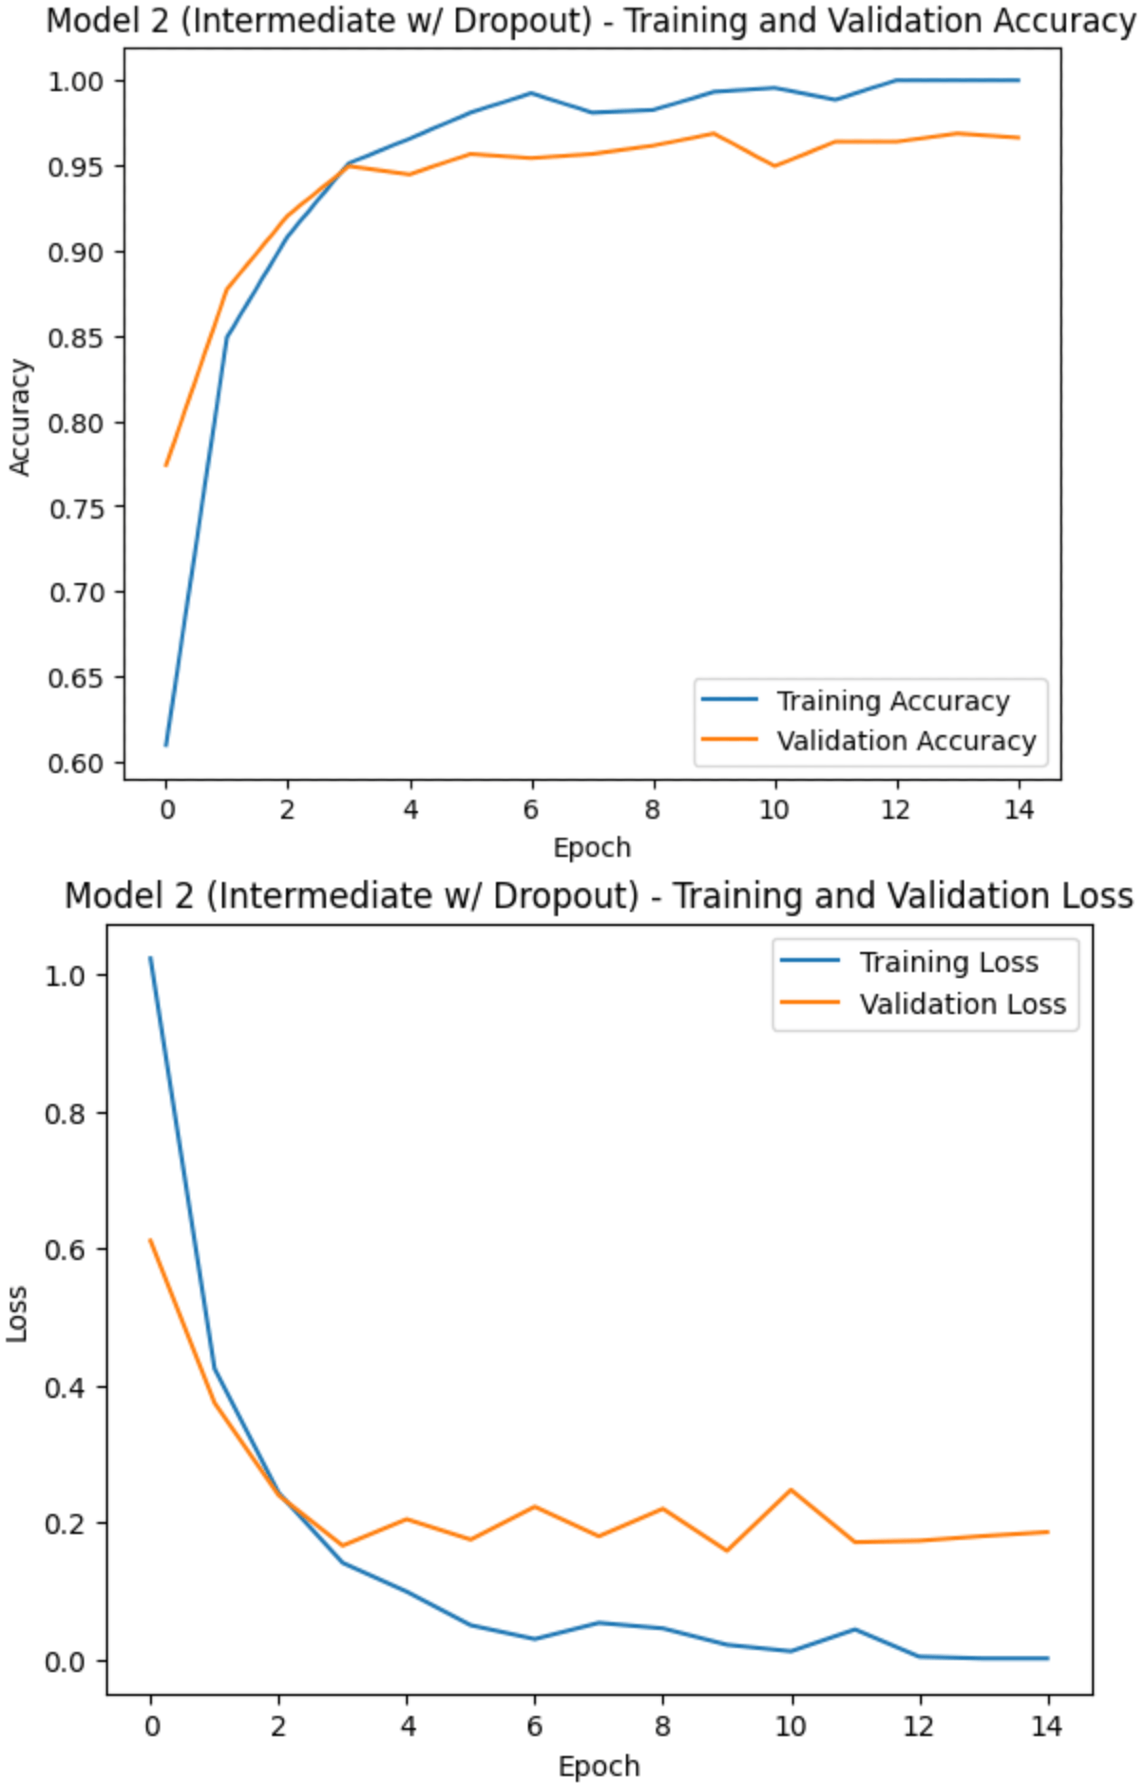
\includegraphics[width=0.9\textwidth]{model2_curves.png}
\caption{Training and validation accuracy/loss for Model 2. The gap between the curves is reduced, showing that dropout has mitigated some overfitting.}\label{fig:model2}
\end{figure}

\subsection{Model 3: The Power of Data Augmentation}
The third model, trained with data augmentation, yielded the best results. It reached a peak validation accuracy of 98.6\%. The training and validation curves in Figure \ref{fig:model3} track each other very closely, indicating that the overfitting problem has been largely resolved. The model's training accuracy is now much more aligned with its validation accuracy, suggesting a well-balanced model with good generalization.

\begin{figure}[h]
\centering
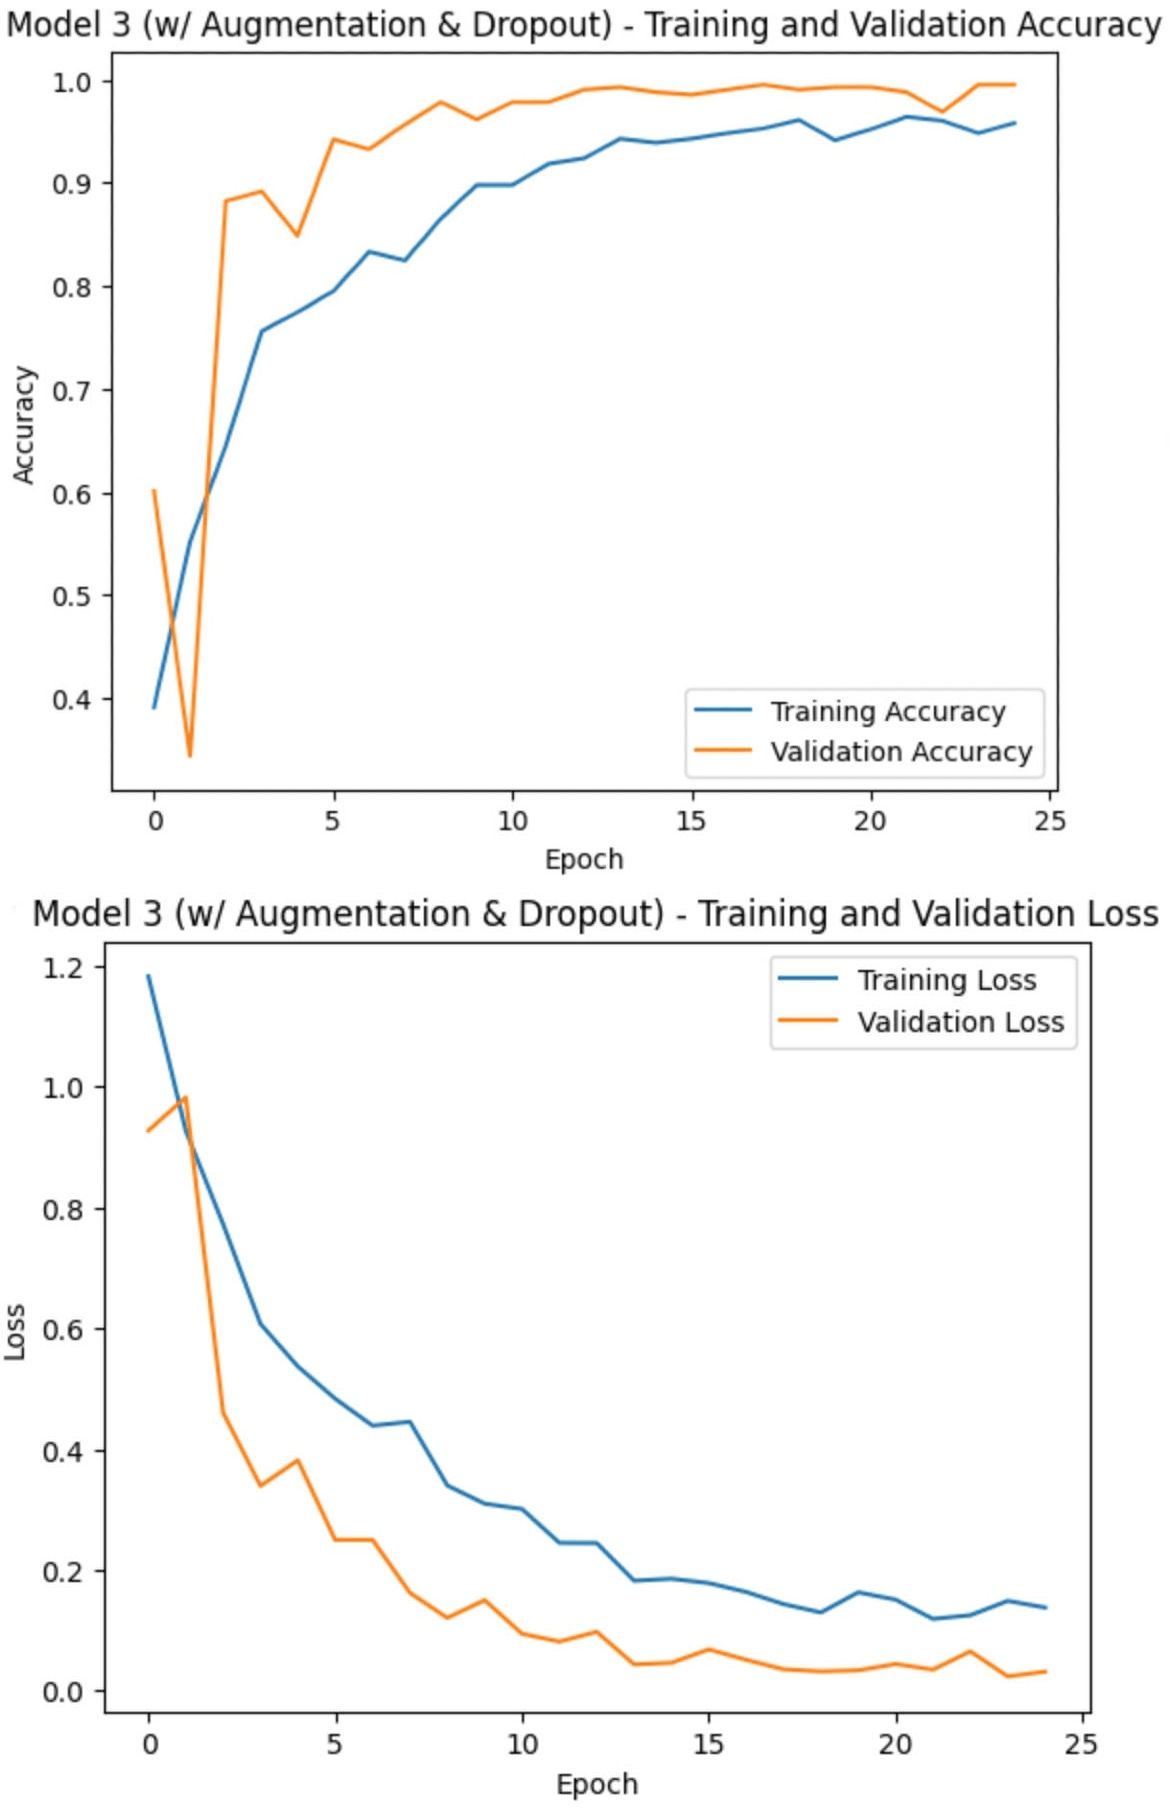
\includegraphics[width=0.9\textwidth]{model3_curves.png}
\caption{Training and validation accuracy/loss for Model 3. The curves are closely aligned, indicating a well-regularized model with excellent generalization.}\label{fig:model3}
\end{figure}

\subsection{Final Model Evaluation}
After hyperparameter tuning, our best model (Model 3 architecture) was evaluated a final time on the held-out test set. This provides an unbiased estimate of its performance on completely unseen data.

The model achieved a **test accuracy of 97.72\%**. The detailed classification report is provided in Table \ref{tab:report}, and the confusion matrix in Figure \ref{fig:cm}.

\begin{table}[h]
\caption{Classification Report for the Final Model on the Test Set}\label{tab:report}%
\begin{tabular}{@{}lcccc@{}}
\toprule
Class & Precision & Recall & F1-Score & Support \\
\midrule
rock     & 0.99 & 0.94 & 0.96 & 141 \\
paper    & 0.95 & 1.00 & 0.97 & 150 \\
scissors & 0.99 & 0.99 & 0.99 & 148 \\
\midrule
Accuracy &      &      & 0.98 & 439 \\
Macro Avg & 0.98 & 0.98 & 0.98 & 439 \\
Weighted Avg & 0.98 & 0.98 & 0.98 & 439 \\
\botrule
\end{tabular}
\end{table}

\begin{figure}[h]
\centering
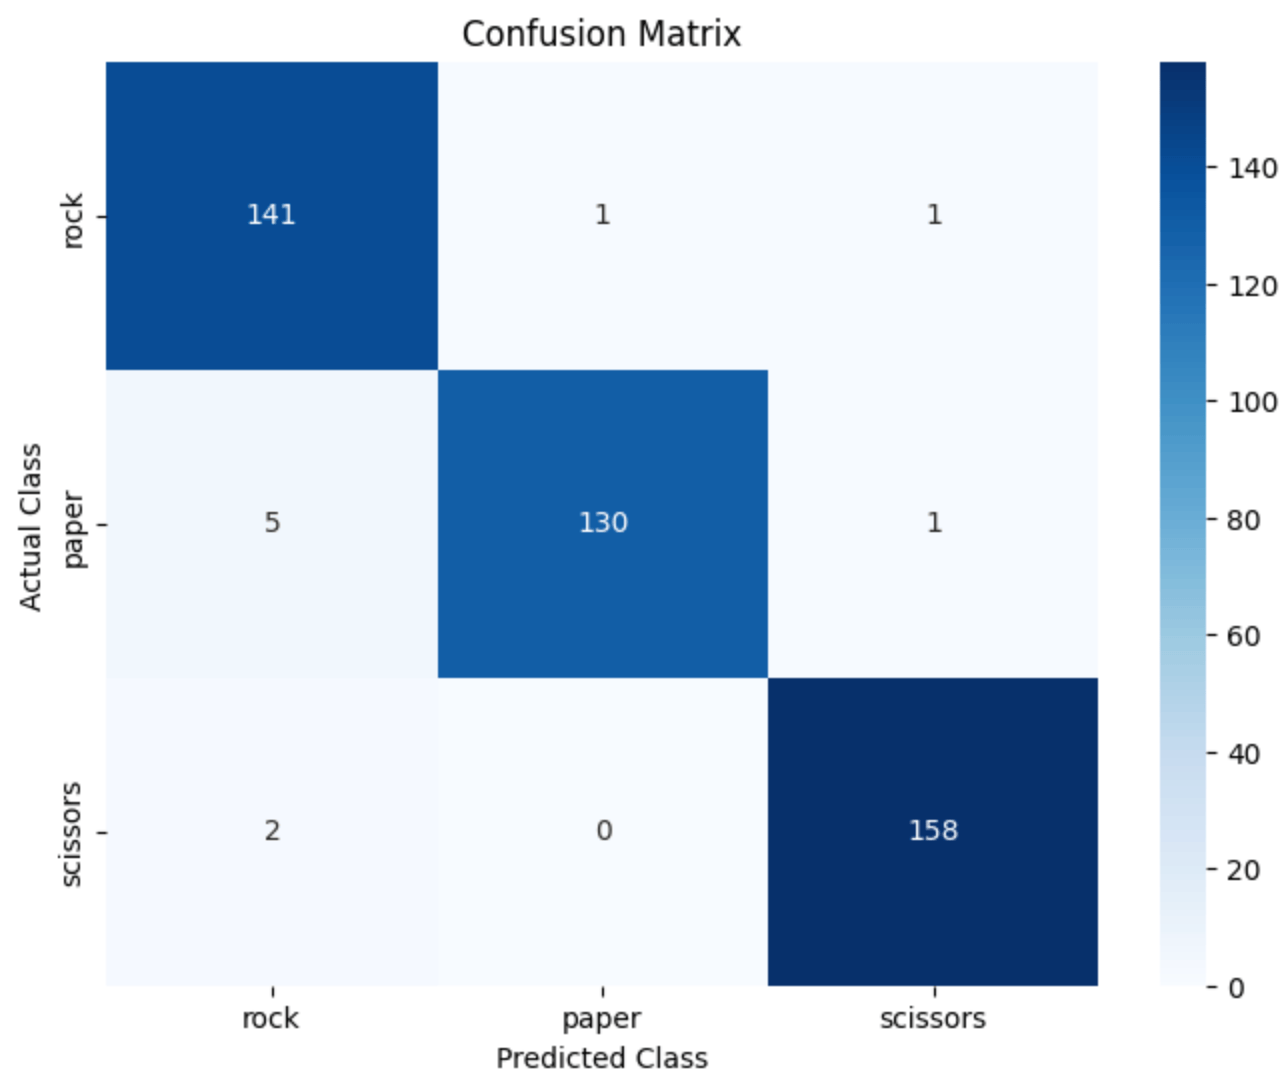
\includegraphics[width=0.6\textwidth]{confusion_matrix.png}
\caption{Confusion matrix for the final model on the test set. The model shows high accuracy across all classes, with the most frequent error being the misclassification of 'rock' as 'paper'.}\label{fig:cm}
\end{figure}

The results show excellent performance, with high precision and recall across all classes. The confusion matrix reveals that the model is highly accurate, with the most notable error being the misclassification of 8 'rock' instances as 'paper'.

\section{Discussion}\label{sec12}

This project successfully demonstrated a structured approach to building a high-performance CNN classifier. The progression from a simple, overfitting model to a well-regularized, generalizable model highlights several key concepts from statistical learning.

The initial baseline model, despite its high training accuracy, was a clear example of high variance. Its inability to generalize was addressed by introducing regularization. Model 2 showed that dropout is an effective technique for reducing variance, forcing the network to learn more robust feature representations. However, the most significant improvement came from Model 3 with data augmentation. By artificially enriching the training data, we forced the model to become invariant to minor changes in position, orientation, and scale, which dramatically improved its generalization and closed the gap between training and validation performance.

The final test accuracy of 97.7\% is a strong result, but the optional generalization test conducted on custom, user-generated images revealed the model's limitations. Performance on these images, which come from a different data distribution (different camera, lighting, etc.), was notably lower. This illustrates the concept of **domain shift**, where a model trained on one distribution may not perform as well on another. It underscores that even a model with a low statistical risk on its test set may not be universally applicable without further adaptation.

\section{Conclusion}\label{sec13}

In this project, we successfully developed a Convolutional Neural Network to classify Rock-Paper-Scissors hand gestures with high accuracy. Through a methodical process of incremental complexity and the application of regularization techniques—namely dropout and data augmentation—we systematically addressed the problem of overfitting and significantly improved the model's generalization capabilities. The final model achieved an accuracy of 97.7\% on an unseen test set, demonstrating the effectiveness of our approach. This work serves as a practical case study in applying fundamental machine learning principles to build robust and effective deep learning systems.

\backmatter

\section*{Declarations}

\begin{itemize}
\item \textbf{Funding:} Not applicable.
\item \textbf{Conflict of interest/Competing interests:} The authors declare no competing interests.
\item \textbf{Ethics approval and consent to participate:} Not applicable.
\item \textbf{Consent for publication:} Not applicable.
\item \textbf{Data availability:} The dataset used in this study is publicly available on Kaggle at \url{https://www.kaggle.com/datasets/drgfreeman/rockpaperscissors}.
\item \textbf{Code availability:} The code developed for this project is available in the author's public GitHub repository.
\item \textbf{Author contribution:} The sole author designed the study, conducted the experiments, analyzed the results, and wrote the manuscript.
\end{itemize}

\begin{thebibliography}{9}

\bibitem{cesa2024smml}
Cesa-Bianchi, N. (2024). *Course Notebook: Statistical Methods for Machine Learning*. University of Milan.

\bibitem{kaggle_rps}
Dr. G. Freeman. (2019). Rock Paper Scissors Dataset. Kaggle. \url{https://www.kaggle.com/datasets/drgfreeman/rockpaperscissors}

\end{thebibliography}

\end{document}